\section{Resultados y análisis}
\subsection{Calor específico a temperatura ambiente}
Tras realizas las mediciones para cada muestra, haciendo uso de la ecuación \ref{eq:masas} se determina el calor específico para cada material consignado en la tabla \ref{tab:cp}:

\begin{table}[H]
    \centering
    \begin{tabular}{|c|c|c|c|c|}
    \hline
        Muestra&T_0 Agua &T_{masa} &T_{eq} &c_{p} (J/g K) \\\hline
        \multirow{4}{*}{Hierro}&21.5 &91.0 &28.1  &0.101 \\
        &21.5 &93.8 &26.8&0.108  \\
        & 22.2& 94.2&  27.4&0.097 \\
        & 22.2& 94.0&  27.0&0.096 \\\hline
        \multicolumn{4}{|c|}{Valor promedio}&0.101\\\hline
        \multirow{4}{*}{Cobre}&22.6 &94.4 &28.0 &0.264  \\
        &22.6 &95.0 &28.0 &0.248 \\
        & 22.9& 94.0&27.7 & 0.216\\
        &22.9 & 94.4& 25.5&0.126 \\
        \hline
        \multicolumn{4}{|c|}{Valor promedio}&0.195\\\hline
        \multirow{4}{*}{Aluminio}&22.1 & 94&26.6 &0.192  \\
        & 21.9&94 &26.1 &0.193  \\
        & 22.0&94 &25.7 & 0.187 \\
        & 21.3& 94& 25.2& 0.207 \\
        \hline
     \multicolumn{4}{|c|}{Valor promedio}&0.214\\\hline
     
    \end{tabular}
    \caption{Medicion temperaturas y cálculo de c_{p}}
    \label{tab:cp}
\end{table}

De este modo,

\subsection{Capacidad calorífica a bajas temperaturas}

\begin{figure}
    \centering
    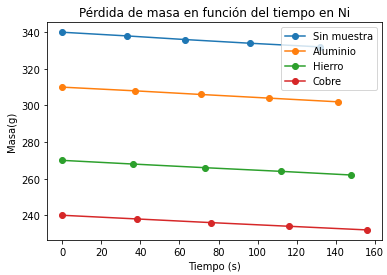
\includegraphics[scale=0.8]{img/nitro.png}
    \caption{Caption}
    \label{fig:my_label}
\end{figure}
\begin{figure}
    \centering
    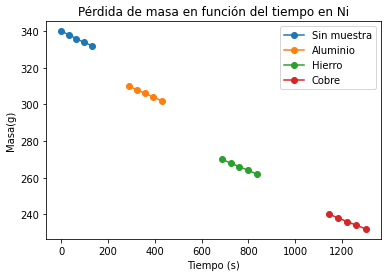
\includegraphics[scale=0.8]{img/nitro2.png}
    \caption{Caption}
    \label{fig:my_label}
\end{figure}